\newpage


\section*{Population Growth and Technological Progress}


\subsection*{The Steady State with Population Growth}

\al{
    \Delta{k} = i - (\delta + n)k 
}

\noindent With the introduction of population growth, the change in capital equation becomes the above. The term $(\delta + n)k$ is 
known as the break-even investment, the amount of investment necessary to keep the capital stock per worker constant. 
To be more specific the equation will be written as: 

\al{
    \Delta(k) = sf(k) - (\delta + n)k
}


\subsection*{The Effects of Population Growth}

\subsection*{Alternative Perspectives on Population Growth}

\section*{Technological Progress in the Solow Model}

\begin{figure}
    \centering
    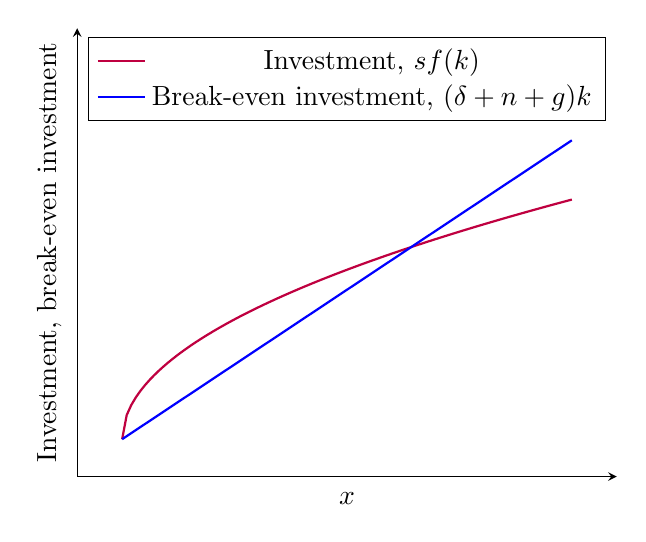
\begin{tikzpicture}
        \begin{axis}[
            axis lines = left, 
            xlabel={\(x\)},
            ylabel={Investment, break-even investment},
            ymin=0, xmax=3.5, ymax=3.5,
            xtick=\empty, ytick=\empty,
            samples=100, domain=0:3.5,
            enlargelimits=true,
            clip=false
        ]
            % Investment function s f(k)
            \addplot [thick, purple] {1.2*x^(0.5)};
            \addlegendentry{Investment, \( s f(k) \)}
            
            % Break-even investment (δ + n + g) k
            \addplot [thick, blue] {0.8*x};
            \addlegendentry{Break-even investment, \( (\delta + n + g) k \)}
  
        \end{axis}
    \end{tikzpicture}

    \caption{Solow Growth Model with Technological Progress}
\end{figure}

\subsection*{The Efficiency of Labor}

\subsection*{The Steady State with Technological Progress}

\subsection*{The Effects of Technological Progress}

\section*{Beyond the Solow Model: Endongenous Growth Theory}

\subsection*{The Basic Model}

\subsection*{A Two-Sector Model}

\subsection*{The Microeconomics of Research and Development}

\subsection*{The Process of Creative Destruction}
